\begin{figure}[t]
\centering
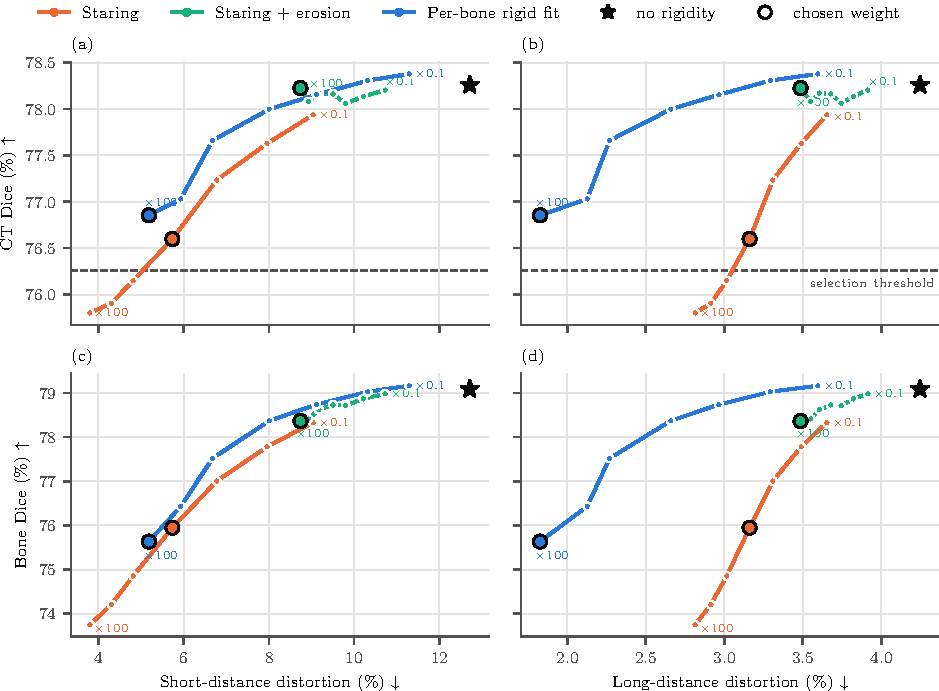
\includegraphics[width=\textwidth]{figures/rigidity.pdf}
\caption{\protect\todo{Draft: first validation sweep (interior-only distortion). After the final sweep: rerun figure\_rigidity.py.} Rigidity weight sweep on the validation set: network trained with the PET losses, IO with the PET terms and one rigidity penalty at $0.1$ to $100$ times its calibrated reference weight (factors at the ends of each line). Top: CT Dice, bottom: bone Dice; left: distortion of short (5--15~mm), right: of long ($\geq$15~mm) within-bone distances, i.e.\ the mean relative change of the distance between point pairs in the same bone. Star: variant without rigidity; dashed (a,~b): selection threshold, one Dice point below it; outlined: weight chosen for the test set (the largest within the threshold, at most $\times100$). Points: patient means.}
\label{fig:rigidity}
\end{figure}
